\documentclass[border=3pt]{standalone}
\usepackage{xcolor}
\usepackage{tikz}
\usetikzlibrary{arrows.meta,decorations.markings}

\definecolor{curveblue}{HTML}{1D4ED8}
\definecolor{accent}{HTML}{BE123C}

\begin{document}
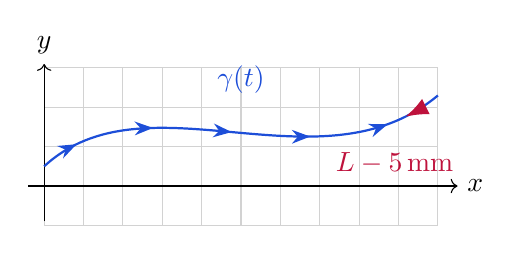
\begin{tikzpicture}
  \draw[gray!35,step=5mm] (0,-.5) grid (5,1.5);
  \draw[->] (-.2,0) -- (5.25,0) node[right] {$x$};
  \draw[->] (0,-.45) -- (0,1.55) node[above] {$y$};

  \draw[curveblue,line width=.8pt,postaction={decorate},
    decoration={markings,
      mark=between positions 5mm and -5mm step 10mm with {\arrow{Stealth}},
      mark=at position -5mm with {\arrowreversed[accent,very thick]{Latex}}}]
    (0,.25) .. controls (1.3,1.45) and (3.5,-.1) .. (5,1.15);

  \node[curveblue,above] at (2.5,1.05) {$\gamma(t)$};
  \node[accent,below] at (4.45,.55) {$L-5\,\mathrm{mm}$};
\end{tikzpicture}
\end{document}
